\part{Architecture de l'application} % (fold)
\label{prt:architecture_ _de_ _l_'_application_}
	
	\section{Composant de l'application} % (fold)
	\label{sec:composant_de_l_application}
	\begin{figure}[h!]
			\centering
		    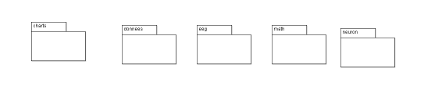
\includegraphics []{../diagramme_classes/packages.png} \\
		    \captionof{figure}{Packages composant l'application}
			\label{fig_pack}
	\end{figure}
	L'application est composée de cinq packages: eeg, math, neuron, charts et donnees. Nous allons donc décrire le contenu de chacun de ces packages ainsi que le rôle des classes qui les composent:
	\begin{itemize}
			
	\item [-] eeg : 
		\begin{figure}[h!]
			\centering
		    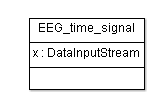
\includegraphics []{../diagramme_classes/eeg.png} \\
		    \captionof{figure}{Classe EEG\_time\_signal}
			\label{fig_eeg}
  		\end{figure}
	 contient la classe EEG\_time\_signal qui contiendra les fonctions concernant le traitement du signal en fonction des données reçues et traitées;
	\item [-] math :
		\begin{figure}[h!]
			\centering
		    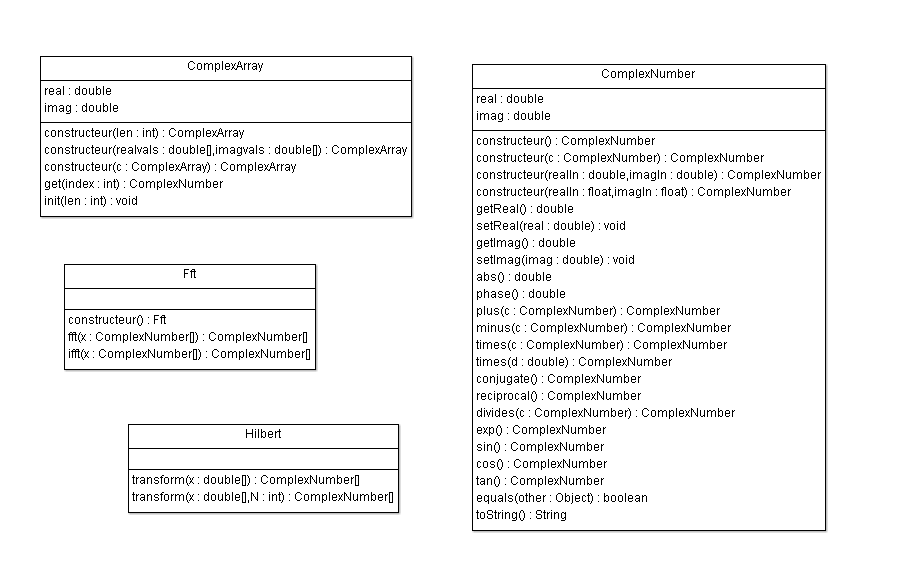
\includegraphics [scale=0.5]{../diagramme_classes/math.png} 
		    \captionof{figure}{Classes pour les calculs mathématiques }
			\label{fig_math}
    		\end{figure} 
	contient toutes les fonctions mathématiques avec la classe ComplexNumber permettant de créer et gérer les nombres complexes, la classe ComplexArray qui permet de stocker les valeurs réelles et imaginaires des nombres complexes, la classe Hilbert qui contient les fonctions concernant les espaces d'Hilbert (extension des espaces euclidiens à des dimensions finies quelconques ou infinies) et enfin la classe Fft qui contient les fonctions en rapport avec la Transformée Rapide de Fourrier(ou Fast Fourrier Transform);
	\newpage
	\item [-] neuron : 
	\begin{figure}[h!]
			\centering
		    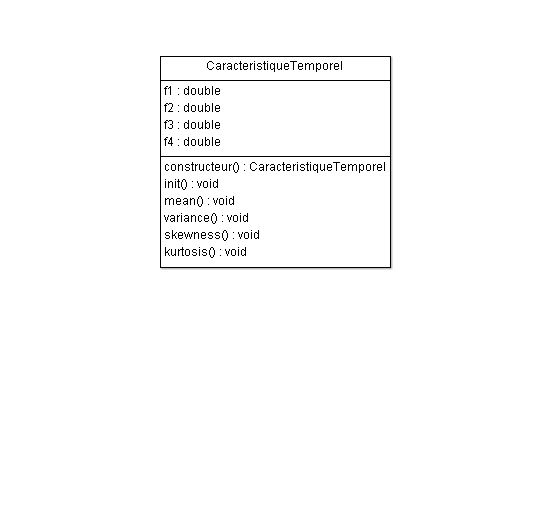
\includegraphics []{../diagramme_classes/neuron.png} \\
		    \captionof{figure}{Classe Caractéristique}
			\label{fig_neuron}
    		\end{figure}
	contient la classe CaracteristiqueTemporel qui contient toutes les fonctions ayant attrait aux caractéristiques temporelles d'un neuronne pour le réseau qui sera par la suite créé. Ces caractéristiques temporelles regroupent notamment la moyenne des données, la variance, etc...;
	\item [-] charts :
	 \begin{figure}[h!]
			\centering
		    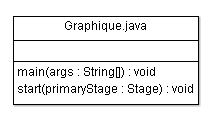
\includegraphics []{../diagramme_classes/charts.png} \\
		    \captionof{figure}{Classe Graphique}
			\label{fig_graph}
			\end{figure}
	 contient la classe Graphique afin de générer les graphiques une fois les résultats obtenus à partir des données grâce à la librairie JFreeCharts;
	\item [-] donnees : 
		\begin{figure}[h!]
		    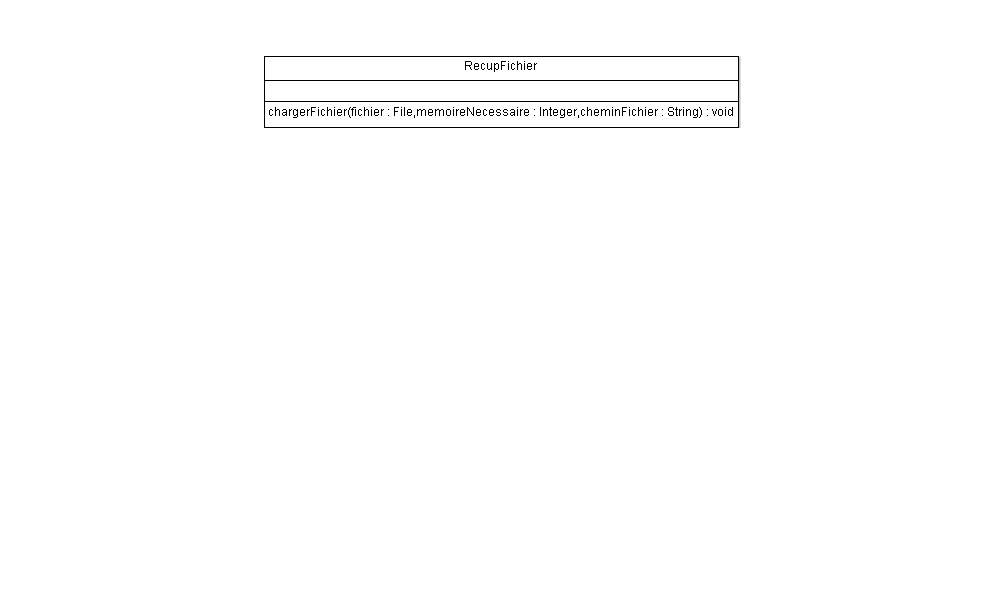
\includegraphics []{../diagramme_classes/donnees.png} \\
		    \captionof{figure}{Classe RecupFichier}
			\label{fig_donnees}
  			\end{figure}
	contient la classe RecupFichier permettant de récupérer la base de données pour la stocker en mémoire afin de permettre au programme de travailler avec.
	
	\end{itemize}
	
	% section composant_de_l_application (end)

	\section{Explication Technique} % (fold)
	\label{sec:explication_technique}
		
		\section{Idéés} % (fold)
		\label{sec:idees}

		
		Nous avons eu l'idée, pour ce projet, de créer un "classifieur" représenté par un réseau de neurones afin d'obtenir des résultats à partir d'un flux de données que nous stockerons en mémoire dans un tableau. Chaque donnée sera représentée par un vecteur. Pour chaque vecteur, chacune de ses dimensions représentera une caractéristique du signal EEG de la personne atteinte que nous chercherons à reconnaître (le tout afin de reconnaître les états tel : lecture, repos, regarder un film, etc...). Nous sommes partis de ces idées là car, lors de nos lectures sur les interfaces cerveau-machine, il s'est avéré que ce mode de traitement du signal est très utilisé .
		
		% section idéés (end)
		\section{Outils} % (fold)
		\label{sec:outils}
		
		Nous avons développé notre application au moyen du langage Java et nous avons utilisé l'IDE Intellij qui est très pratique car très ergonomique et très intuitif. 
		Deplus nous avons utilisé Git comme gestionnaire de version, le code étant hébergé sur les serveurs de Github. De surcroît nous avons utilisé JavaDoc pour générer un documentation du code.
		Par ailleurs, nous avons inclus la librairie JFreeCharts pour réaliser des graphiques sans les contraintes de la bibliothèque Swing pour créer des interfaces ainsi que l'extension LaTex afin de rédiger plus facilement nos rapports directement au sein de l'IDE.
		Par ailleurs, nous avons utilisé le logiciel argoUML pour réaliser le diagramme de classes de l'application et OpenOffice Draw pour réaliser l'organigramme.
		
		% section outils (end)
		\section{Algorithmes} % (fold)
		\label{sec:algorithmes}
		 Par rapport à notre avancement courant, les algorithmes les plus intéressant à présenter sont la fft\footnote{Fast Fourrier Transform} et la transformé de Hilbert qui utilise la fft . \\ 
		 La fft est un algorithme de calcul de la transformation de Fourrier discrète il nous sert lors de la partie de post-traitement du signal, mais aussi dans la transformée d'Hilbert.\\
		 La transformée d'Hilbert est utilisé dans le traitement du signal pour passer le signal réel dans le domaine complexe d’où la classe ComplexNumber. Cette transformée est utilisé lors des calculs de caractéristique temporelles .

		% section algorithmes (end)
	% section explication_technique (end)
% part architecture_ _de_ _l_'_application_ (end)